\chapter{Introduction}\label{ch:introduction}
\section{Overview}
The goal of this Master-Thesis project is to extract structured information from unstructured text and store this information in a Knowledge Graph to facilitate information retrieval.
The unstructured text are financial news articles and the target information to be extracted is information about certain corporate entities or companies.

To extract the information, an \emph{Information Extraction Pipeline} is built that contains three main components:

\begin{figure}[H]
	\centering
	
\includegraphics[width=1.0\textwidth]{Assets/pipelineAll}
	\caption{Information Extraction Pipeline}
	\label{fig:infoextract}
\end{figure}


\begin{itemize}
	\item \textbf{NER}: A Named Entity Recognition component that identifies the desired company names in the text
	\item \textbf{Coreference Resolution}: A \gls{coref_resolution_definition} component that detects references to previously identified company names
	\item \textbf{Topic Modelling}: A Topic Modelling component that classifies those sentences in the text, that contain company names and their coreferences, into different topic classes
\end{itemize}

The \emph{Information Extraction Pipeline} yields sentences that contain company names, their \glspl{coref_definition} and the respective topic for each of these sentences.
This information is then stored in a neo4j \cite{neo4j} Graph database according to the following schema:

\begin{figure}[H]
	\centering
	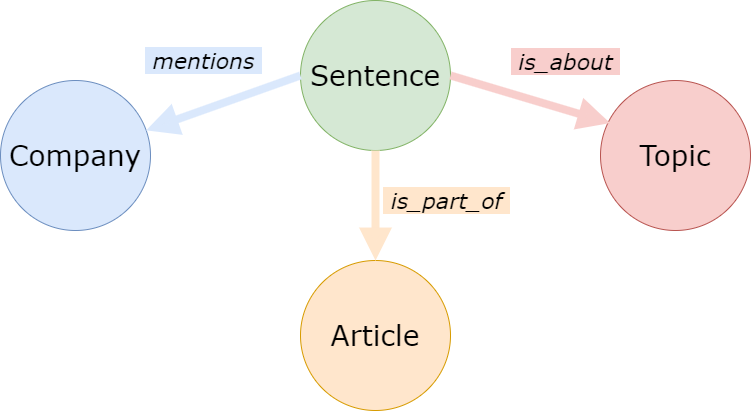
\includegraphics[width=0.85\textwidth]{Assets/kg_schema}
	\caption{Knowledge Graph Schema}
	\label{fig:kg-schema}
\end{figure}

There are three Node types in the Knowledge Graph:

\begin{itemize}
	\item \textbf{Sentence}: the \emph{Sentence} in which a \emph{Company} is mentioned
	\item \textbf{Topic}: the \emph{Topic} or overarching theme of this \emph{Sentence}
	\item \textbf{Company}: the \emph{Company} entity whose name is mentioned in the \emph{Sentence}
	\item \textbf{Article}: the \emph{Article} of which the \emph{Sentence} is part of
\end{itemize}

A \emph{Sentence} Node thus has three relationships to other Nodes in the Knowledge Graph:

\begin{itemize}
	\item \textbf{is\_about}: a \emph{Sentence} is about a certain \emph{Topic}
	\item \textbf{is\_part\_of}: a \emph{Sentence} is part of an \emph{Article}
	\item \textbf{mentions}: a \emph{Sentence} mentions a \emph{Company}
\end{itemize}

This structured representation of the unstructured text does not only allow for fast retrieval of concrete information, but can also reveal complex relationships between multiple companies, topics and articles.

The stored information can be retrieved via \gls{cypher} queries that can also be generated by an \gls{llm}-based \gls{graph-bot} that first converts human text to \gls{cypher} queries and then the results back to human-readable text.

\section{Thesis and Code}\label{sec:domain-focus}
This Master-Thesis consists of two separate parts, the written thesis and the accompanying Python code.

\paragraph{Python Code}
The Python code can be found in the following GitHub repository:
\begin{center}
	\textbf{\url{https://github.com/rainergo/UASFRA-MS-Thesis}}
\end{center}
The code could be used as a template for a production use case, but mainly serves to support this Master-Thesis and to present the process rather than the result.\\
All functionalities of the code are aggregated and condensed in the Jupyter Notebook
\begin{center}
	\emph{MAIN.ipynb}
\end{center}
located in the root directory of the repository and explained in Appendix \ref{ch:explanation-of-main-file}.
This Notebook runs the entire pipeline from text to Knowledge Graph.

\paragraph{Target Use Case}
The Python code is targeted at a user with a particular focus on financial news of publicly listed European companies in German language.
This focus is driven by my professional background in finance and personal interest in this field.

\section{Thesis Outline}\label{sec:thesis-outline}
This thesis will be divided into multiple chapters.
In the chapter after this introduction, I describe the source and nature of the text data.\\
Thereafter, I will describe the spacy \cite{spacy} Python library and how it was used, followed by an introduction to text representation.\\
In the fourth chapter, I start with a description of Named Entity Recognition (\gls{ner}) and how that pipeline component was implemented in code.\\
The same approach applies to the \gls{coref_resolution_definition} and Topic Modelling chapters thereafter.\\
In the Knowledge Graph chapter, I show how the previously extracted data is fed into the neo4j database and how information retrieval algorithms can reveal some complex relations between news articles, companies and topics.\\
I conclude with what I learned from this project and where in hindsight I would approach tasks differently.